%%%%%%%%%%%%%%%%%%%%%%%%%%%%%%%%%%%%%%%%%%%%%%%%%%%%%%%%%%%%%%%%%%%%%%%%%%%%%%%%
\chapter{Generating Feedback}\label{sec:fb}

\begin{chapterBody}

\begin{figure}[ht]
    \centering
    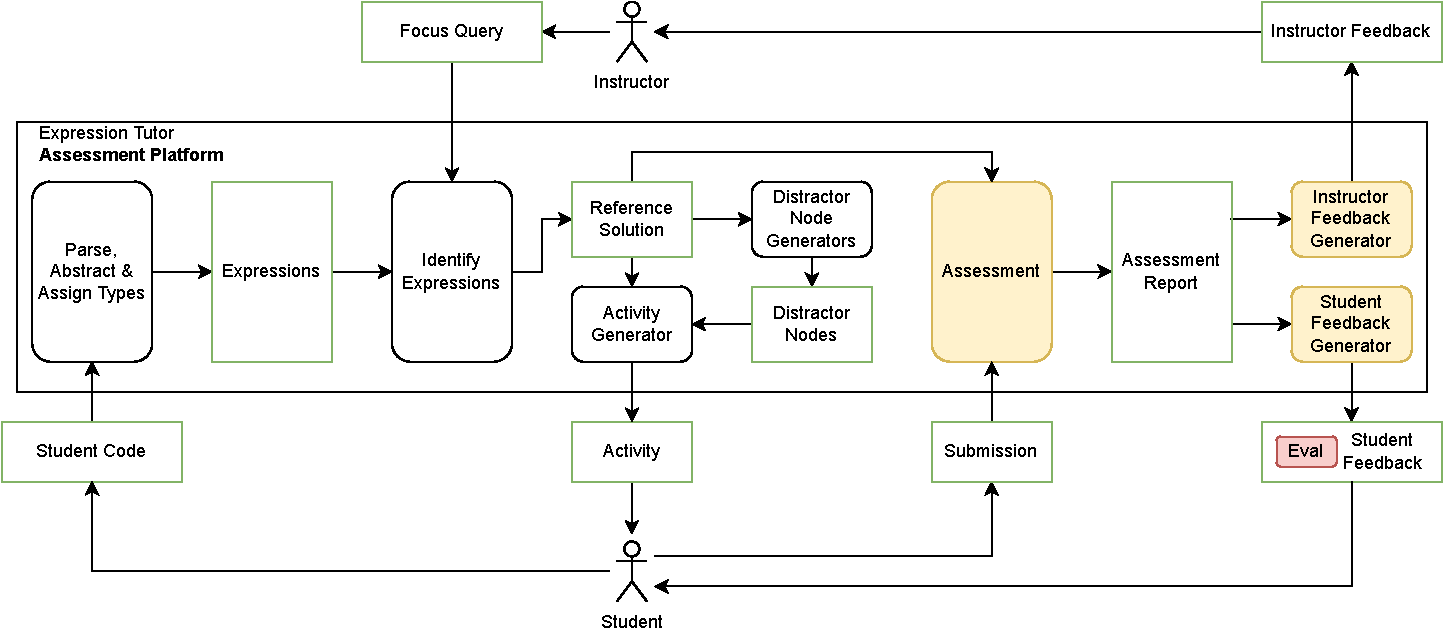
\includegraphics[width=\textwidth]{res/7/et_loop_assessment.pdf}
    \caption{Assessing a student's submission against its reference solution to
produce feedback.}
    \label{fig:fb-intro-loop}
\end{figure}


Another situation in which automation is required to deal with large number of
students, is assessing the submissions and providing feedback.
To generate valuable feedback for both students and instructors.
The two have different needs: instructors find more useful aggregate results
to understand recurring issues and overall performance of the students with
regards to the learning goals the Expression Tutor Activity was supposed
to work towards to.
On the other hand, students find more useful more detailed feedback that
regards only their submission, what they did right or wrong and how they
can improve.

To provide both of these experiences, we build an automated assessment
system that compares each activity against its reference solution.
The assessment system can be described as a function that takes a
pair of expression tree diagrams (one student submission and one
respective reference solution) and produces an assessment report
(\textbf{Section~\ref{sec:fb-assess}}).

Formally, we need to devise a function that takes two expression tree
Diagrams (one for the student's submission and one for the reference
solution) and produces an assessment report, as highlighted in
\textbf{Figure~\ref{fig:fb-intro-loop}}.

\[
\text{assessment}:
\left(\text{ExprTreeDiagram}, \text{ExprTreeDiagram}\right)
\rightarrow
\text{AssessmentReport}
\]

For students we can take the assessment report of their submission
and generate formative feedback (\textbf{Section~\ref{sec:fb-ff}}),
while for instructors, we can aggregate multiple assessment reports and
generate feedback for instructors (\textbf{Section~\ref{sec:fb-sf}}).
We can formalize the two feedback generation processes as two functions
that take an assessment report and produce the appropriate feedback.

\[
\text{studentFeedbackGenerator}:
\text{AssessmentReport}
\rightarrow
\text{StudentFeedback}
\]


\[
\text{instructorFeedbackGenerator}:
\text{AssessmentReport}
\rightarrow
\text{InstructorFeedback}
\]

\section{Assessing a Submission}\label{sec:fb-assess}

At the core of the assessment operation is the comparison between the
student's submission and the respective reference solution.
By interviewing different instructors and asking them to grade different
submissions of Expression Tutor activities, it becomes apparent how there is
little to no common ground on how they should be evaluated. Instructors assign
different weights to the various aspects of each submission. Some times, certain
aspects that may be deemed important by some are not even considered by others.
In general, there is some consensus on the strong importance of the correctness
of the nodes (Section~\ref{sec:fb-assess-nodes}) and whether the linearization 
(Section~\ref{sec:fb-assess-linearization}) of the submission matches the 
linearization of the reference solution.
For this reason, we decide to adopt a number of heuristics to come up with a
reasonable assessment of an expression tree activity submission.
The most simple yet effective strategy to assess a submission is to compare
each  \textit{component} of the student's submission against the
\textit{supposed–respective component} in the reference solution. While
this seems to be a simple process on the surface, there are a number of nuances
due to the nature of expression tree diagrams and the mistakes this data
structure is capable of capturing as opposed to a plain tree–shaped
data structure, as illustrated in Figure~\ref{fig:bg-et-etd-incorrect}.

\subsection{Selecting the Main Connected Component}\label{sec:fb-assess-mc}

The Expression Tutor platform operates on the expression tree diagram data 
structure \hfill\break (Section~\ref{sec:bg-rw-le-et}), which allows more
mistakes to be captured.
Among those, we find the possibility of representing more than one connected
component, something that would not be possible if the data structure was simply
an \textit{expression tree}.

It is not uncommon to run into  submissions of students who draw more than one
expression tree while solving an Expression Tutor activity. When such a thing
happens, it becomes harder to perform automated assessment operations.
Moreover, it is not desirable to expect students to manually delete all the
unused distractor nodes. It is a both time–consuming and \textit{dangerous}
operation. If a student deletes one node and then realizes that it was actually
needed, they would have to start solving the task from the beginning again as it
is not possible for them to create new nodes.
To compare the expression tree diagram of the reference solution, which is
assumed to also be a valid expression \emph{tree}, one connected component from
the student's submission  must be selected.

One approach to solving the problem of selecting the main connected component
would be selecting the one that includes the root node.
When completing an Expression Tutor activity, students are expected to identify
the root node of an expression tree by double–clicking on it. This marks the
selected node with a star to signify it is the root node.

Unfortunately, not only it is possible for students to submit without selecting
a root node, but it cannot be assumed that the root of an expression tree
diagram is actually the root of a tree.
A node that is inside a tree, or even a leaf could potentially be selected as
the root.
Moreover, students may compose multiple connected components, one of which is the
correct one, but pick a node of another one as the root.
Or they might even \textit{accidentally} set an otherwise unused node as the
root. In such situations, the sub–optimal selection of the main connected
component leads the rest of the assessment process to produce less useful
feedback.
\textbf{Figure~\ref{fig:fb-assess-mcc-wrong-root}} illustrates a real student's
submission in which the root node is set to an otherwise unused node. The
original heuristic would just select a connected component made of just one one
and discard the actual correct tree of the expression.
For these reasons, it cannot be assumed that being the root of an expression tree
diagram has much weight in the context of selecting the main connected component.

To select the main connected component, first we select the biggest one among
all of those found within the expression tree Diagram. In case of multiple
\textit{biggest} connected components with the same size, priority is given to
the one that contains the root node (if one such connected component exists).
This strategy, prevents situations such as that of
Figure~\ref{fig:fb-assess-mcc-wrong-root}.
This strategy overcomes the problem of accidental root node selection on
unused nodes. On the other hand, there can still be situations in which the
selected connected component is not the correct one due to the sheer amount of
possible situations that can be represented by the expression tree diagram
data structure.

\begin{figure}[ht]
    \centering
    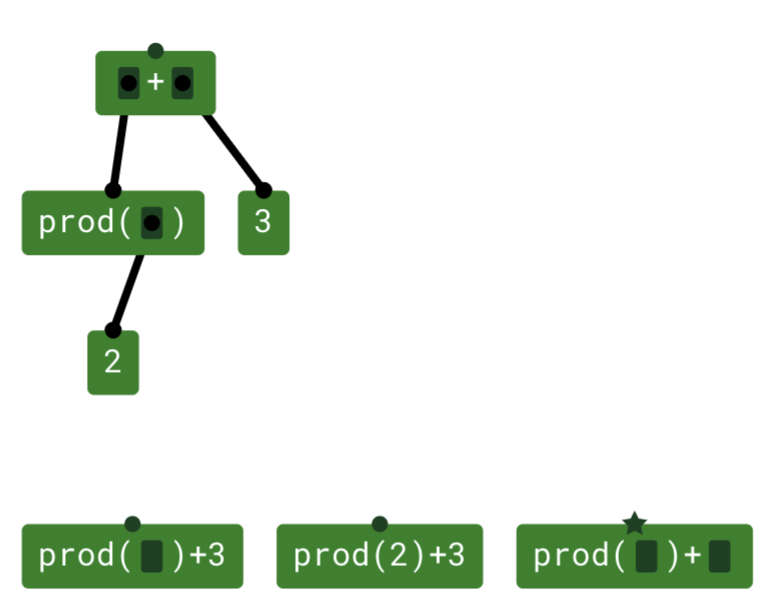
\includegraphics[width=0.5\textwidth]
                    {res/7/assessment_mcc_wrong_root_example.png}
    \caption{Example of a student's submission in which the root node is
set on the otherwise–unused node
\lstinline[language=etl]{("prod" "(" () ")" "+" ())}.}
    \label{fig:fb-assess-mcc-wrong-root}
\end{figure}

\subsection{Correctness of the Tree Structure}\label{sec:fb-assess-tree}

Now that we have selected the main connected component to assess, we begin by 
checking whether it is also a valid tree. If we can establish that the target
of the assessment is a valid tree, just like the reference solution, then
comparing the two becomes much easier as it would be possible to leverage
existing tree comparison algorithms.

To understand whether a given expression tree diagram (or a subset of it) is
a valid tree, we define a number of properties that must all be satisfied to
make such a claim:

\begin{enumerate}
    \item The diagram should not have multiple roots. There can exist only one
node with a top plug that is \emph{not} connected to another node through an edge. That node
would be the root of the tree.
    \item Holes should not be connected to other holes. Holes may only be
connected to top plugs of other nodes.
    \item Top plugs of nodes should not be connected to top plugs of other
nodes. Top plugs may only be connected to holes inside of other nodes.
    \item All holes should be \textit{filled} (connected). There can be no
\textit{unused} hole. Holes represent operands and arguments, and expressions
in syntactically correct programs cannot have \textit{holes}.
    \item No two edges should start or end at the same place. This may be
generalized by stating that all plugs can be used at most once. This includes
both top plug of nodes and plugs inside holes (see Section~\ref{sec:bg-rw-le-et}
for implementation details about the expression tree diagram data structure).
    \item If a \textit{root} node is defined, then it must be the only node
with a non-connected top plug.
\end{enumerate}

We require that all properties are satisfied to perform a more advanced
assessment on the tree. Although, an exception is made for property 4.
If the main connected component satisfies all properties but the fourth one,
then we can replace the unplugged holes with special markers and still consider
the connected component a valid tree.

\subsection{Correctness of Nodes}\label{sec:fb-assess-nodes}

To determine the correctness of the nodes, we consider the two sets of nodes:
one from the main component of the student submission diagram (\texttt{S}) and
the set from the reference solution diagram (\texttt{R}).

\begin{figure}[ht]
    \centering
    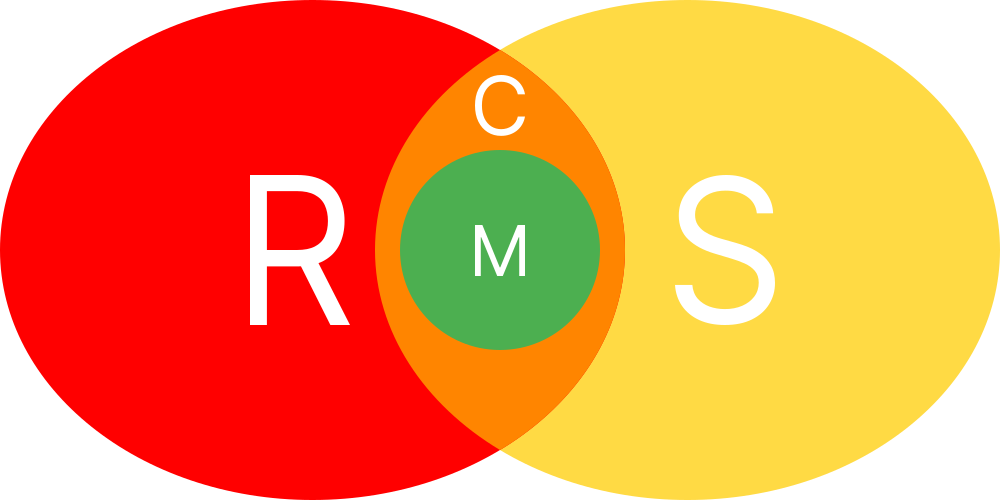
\includegraphics[width=0.4\textwidth]{res/7/assessment_correctness.png}
    \caption{Correctness sets of nodes assessment.}
    \label{fig:fb-assess-correctness-sets}
\end{figure}

We consider nodes to be correct if they exists in both the $ S $ and $ R $
sets. In other words when they belong to the set $ C = S \cap R $ operation,
depicted with the color orange in
\textbf{Figure~\ref{fig:fb-assess-correctness-sets}}. 

There exists another set, $ M \subseteq C $. Nodes found in the $ M $
(which stands for \textit{match}) set are those for which it was possible to
find a univocal correspondence between the two set of nodes, from the submission
to the reference.
If the previously–checked properties that define whether the expression tree
diagram made of the main component of the student's submission is a tree, then
we may employ a tree–edit–distance algorithm to accomplish this task.

A tree–edit–distance algorithm, such as the one proposed by 
\citet{zhang_simple_1989}, can provide a sequence of operations that must
be performed on a \textit{source} tree to transform it into a \textit{target}
tree. These operation are divided in three different categories. Given
a node \texttt{a} in the source tree (student's submission) and a node
\texttt{b} in the target tree (reference solution), the following operations
are possible:

\begin{enumerate}
    \item \texttt{INSERT}: ``insert a node. A consecutive sequence of siblings
among the children of \texttt{a} become the children of 
\texttt{b}.''~\cite{zhang_simple_1989}
    \item \texttt{DELETE}: ``delete a node. All children of the deleted node
\texttt{b} become children of the parent \texttt{a}.''~\cite{zhang_simple_1989}
    \item \texttt{CHANGE}: ``change one node label to 
another.''~\cite{zhang_simple_1989}. In the case of an expression tree
diagram, rather
than the label of the node, we change the list of \texttt{NodeContentElements}
within the node.
\end{enumerate}

We consider all nodes that were \texttt{INSERT}'ed as nodes that belong only
to the $ R $ set. This is necessary, because to \textit{transform} the
student's submission into the reference solution, a \textit{missing} node had
to be added.
On the other hand, all nodes that were \texttt{DELETE}'d are classified as
belonging only to the $ S $ set. Meaning that all those nodes are not part of 
the tree of the reference solution and thus they had to be removed to 
accomplish the transformation to the target tree.
Finally, the nodes that were \texttt{CHANGE}'d need additional check
to determine to which set they belong. If the contents of the two nodes
\texttt{a} and \texttt{b} are found to be equal, it means that there is
a bijective correspondence between the two, so they belong to the
$ M $ set. Otherwise, the two nodes \texttt{a} and \texttt{b} belong to the
$ S $ and $ R $ set respectively.

A limitation of the Tree-Edit-Distance (TED) approach to perform assessments
is that the algorithm may prefer to remove and re-add later a certain node
to minimize the edit cost. This can lead to \textit{worse} assessment
results than what one would expect.
The only way to reliably work around this issue is to check the multiplicity
of the nodes: if two matching candidates have the same contents and 
multiplicity exactly one (1), then it is safe to put them in the $ M $
(match) set as there can be no ambiguity as to their correspondence.
If either node has multiplicity greater than one, then there is no reliable way
to know which node corresponds to which, so those are not put in the \texttt{M}
set, but rather in the $ C $ (correct) set only. One such example of
a tree with different nodes with multiplicity higher than 1 can be seen in
\textbf{Figure~\ref{fig:fb-assess-multiplicty}}. The $ M $ set is only
utilized for the assessment of nodes, and not for assessment of types and
edges since for those there is no room for correctness ambiguity such as the
one found for nodes assessment.

\begin{figure}
    \centering
    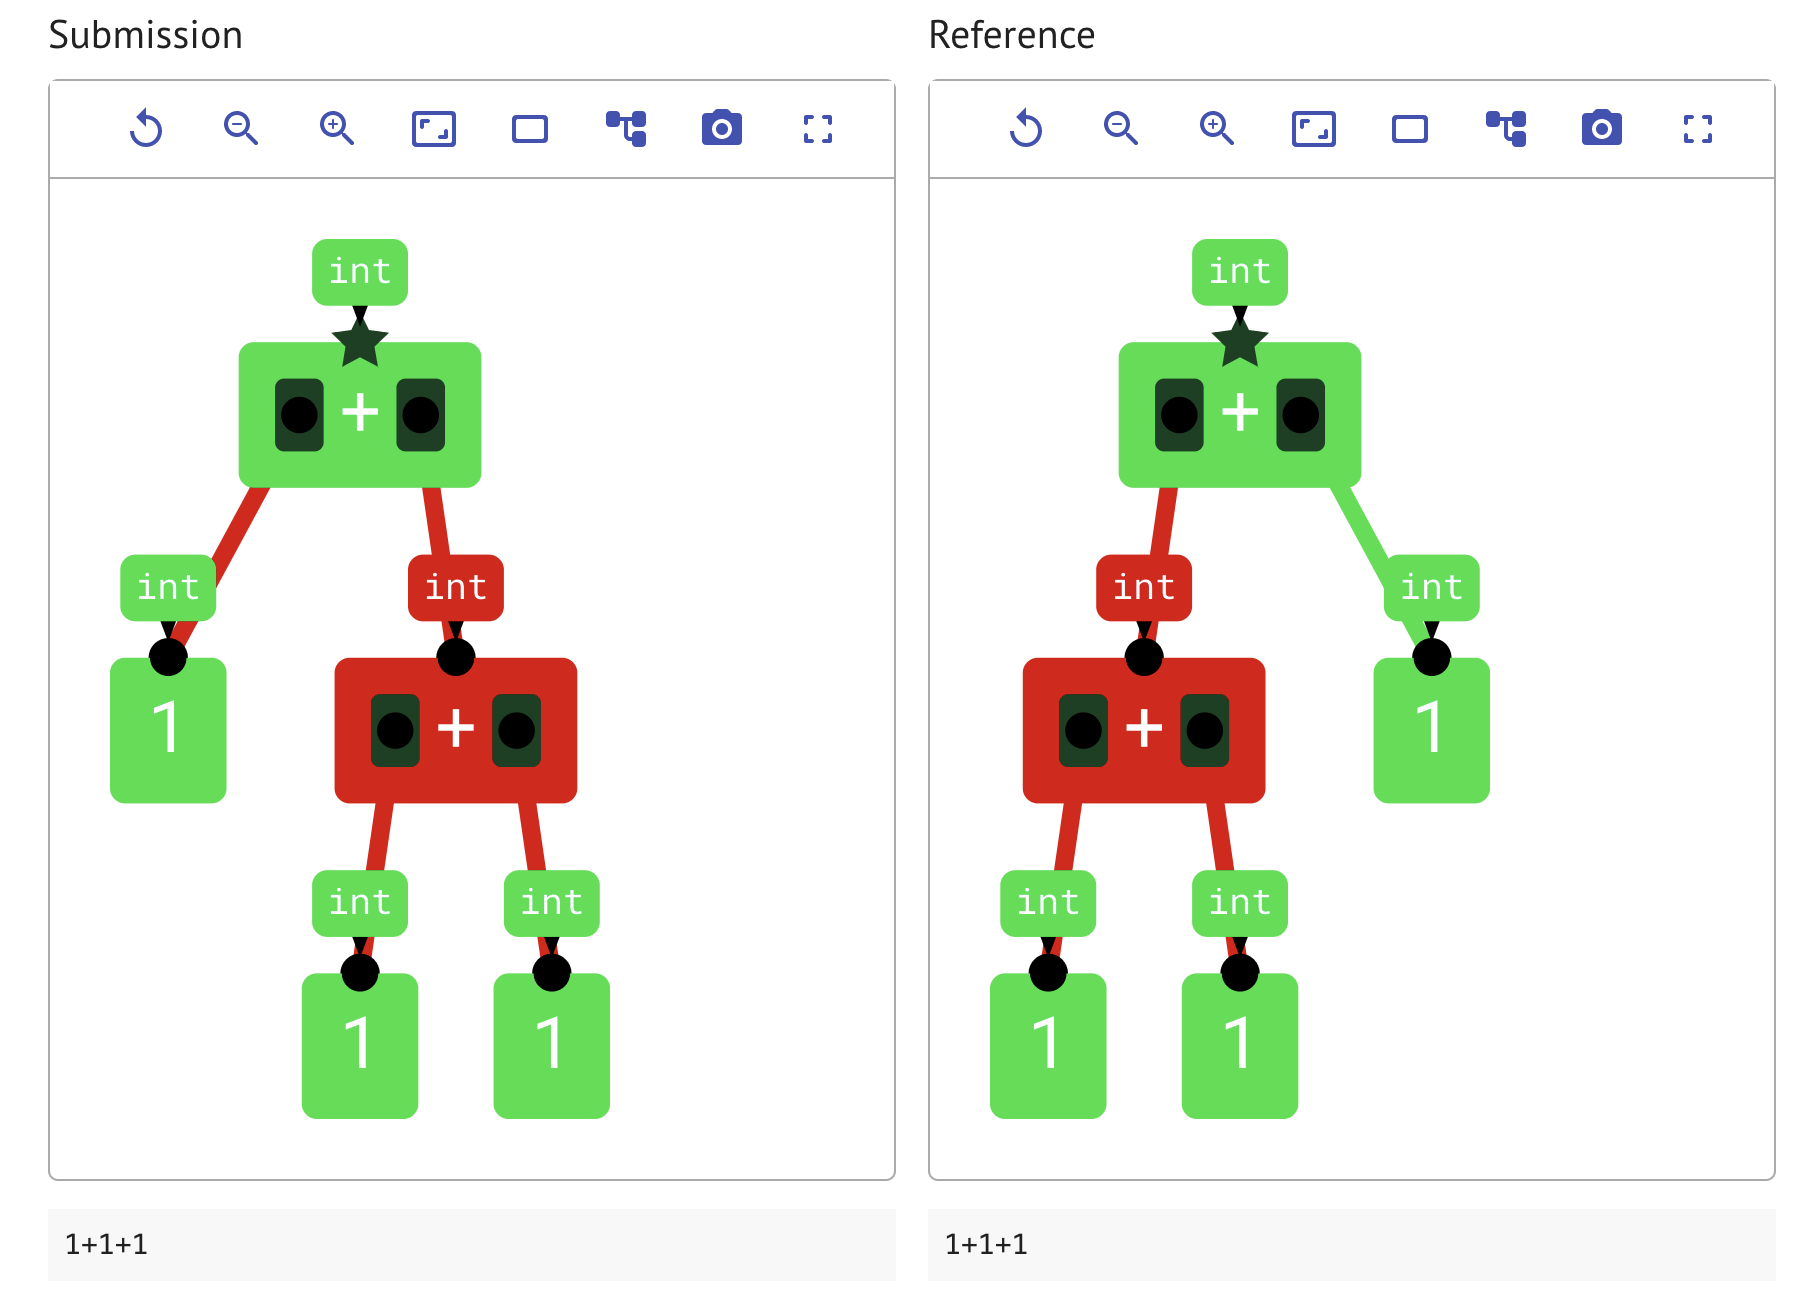
\includegraphics[width=0.8\textwidth]
                    {res/7/assessment_multiplicity.png}
    \caption{Assessment of a tree with multiple nodes with multiplicity higher
than 1. Only the nodes in the $ M $ set are colored in green, while those
in red belong to the $ C $ set.}
    \label{fig:fb-assess-multiplicty}
\end{figure}

The \textit{incorrect} nodes are divided in two categories:
\begin{enumerate}
    \item Nodes present in the student's submission but not in the reference
solution ($ S \setminus R $, marked in yellow in
Figure~\ref{fig:fb-assess-correctness-sets}). We call this set 
\texttt{incorrectSub} (incorrect in submission)
    \item Nodes present in the reference solution but not in the student's
submission ($ R \setminus S $, marked in red in
Figure~\ref{fig:fb-assess-correctness-sets}). We call this set 
\texttt{incorrectRef} (incorrect in reference)
\end{enumerate}

\subsection{Correctness of the Type of the Nodes}\label{sec:fb-assess-types}

The type of a node may be considered correct if and only if the node belongs
to the aforementioned $ M $ set and the non-empty value of the type annotations
of the two matching nodes (one from the reference and one from the submission)
are equal.

\subsection{Correctness of the Edges}\label{sec:fb-assess-edges}

An edge may be considered correct if and only if it connects two different
nodes that both belong in the $ M $ set. To do so, the ids of the two
plugs that compose the edge should match according to the mappings generated
while producing the $ M $ set.
Edges connecting a correct node to an incorrect node are considered
incorrect since the presence of an edge does not provide any additional
meaningful information about the understanding of the correct expression
tree from the student.

\subsection{Correctness of the Root Node}\label{sec:fb-assess-root}

The root node may be assessed by looking at two properties:

\begin{enumerate}
    \item \texttt{set}: whether the submission defines a root node or not.
    \item \texttt{correct}: whether the root is correct, which happens when:
    \begin{enumerate}
        \item The root node is set.
        \item The node marked as root matches the root node of the 
reference solution according to the same criteria applied during the nodes 
assessment.
    \end{enumerate}
\end{enumerate}

\subsection{Diagram Coloring}\label{sec:fb-assess-color}

As a quick and effective way to convey which elements of an expression tree 
diagram are assessed as correct and which are not, the assessment
system includes in the report information that details which set -
among $ S $, $ R $ and $ C $ (and $ M $ for nodes) of
\textbf{Figure~\ref{fig:fb-assess-correctness-sets}}) each node, each
node type and each edge belong to.
This information can then be used by some user–facing interface, such
as the Expression Tutor front–end, to color the original expression tree diagram.

The diagram coloring strategy adopted on the Expression Tutor website
simply uses the color green to represent the types and edges that belong
to their $ C $ set and the nodes that belong to the $ M $ set.
All the other elements of the main connected components are colored red
due to either ambiguity or straight incorrectness.

All the elements of the expression tree diagram that are not part of
the selected main connected component are grayed out to communicate
to the user that they were not considered during the assessment process.

\subsection{Linearization Assessment}\label{sec:fb-assess-linearization}

There exists an interesting class of wrong submissions, which are the ones
that, when serialized, would produce the same code as the
\textit{linearization} of the reference solution. One simple example is
illustrated in \textbf{Figure~\ref{fig:fb-assess-linearization-example}}.

The assessment system includes in the report the \textit{linearization}
of both the reference solution and the student's submission.

We define \textit{linearization} as the flat, type-less and value-less string
representation of an expression tree diagram instance which also happens to
be a valid tree (with respect to the properties defined in
Section~\ref{sec:fb-assess-tree}).

Comparing the linearizations is useful to understand whether a solution is
wrong for example, because of incorrect understanding of operator precedence
or inlining or extracting of pieces of nodes.

\begin{figure}[ht]
    \centering
    \includegraphics[width=0.3\textwidth]
                    {res/7/assessment_linearization_example.png}
    \caption{Two different trees for the expression \texttt{1*2+3} that have the
same linearization, but only one of them is \textit{right}.}
    \label{fig:fb-assess-linearization-example}
\end{figure}

To perform the linearization of a tree, it is necessary to have a ``root node''
from which it is possible to start to walk from, so that all nodes connected
to it are captured.

The difficulty of computing the linearization of a given Expression Tree has to
do with the precedence and associativity rules of the programming language.
One such example would be expressions that make use of parentheses, such as
\lstinline{(1+2)*3}. 
The approach we adopt consists of completely disregard any parentheses that are
just used to avoid notational ambiguity over the order in which expressions are
evaluated. This could lead to \textit{incorrect} linearizations by design, but
would still be useful as they would allow to check whether the
student's submission and the reference solution have the same tokens in the same
order.

For example, for the expression \lstinline{(1+2)*3}, the linearization we produce
is \lstinline{1+2*3}, which in the Java programming language would produce a 
different tree compared to the original expression. But since both the submission
and the reference solution would be \textit{incorrectly} serialized in the
same way, this strategy still accomplishes its goal of checking whether
the tokens in the tree are identical in contents and order.

This approach also covers the situation in which students explicitly
include parentheses that should not be part of the expression tree because
the reference solution is created by using the AST of the source code
(Section~\ref{sec:bg-rw-le-et-es}), and ASTs themselves omit parentheses.



\subsection{Grade}\label{sec:fb-assess-grade}

We compute a \textit{grade} value for the given submission to include in the
assessment report. This value is computed with the goal of quantifying the
correctness of a student's submission rather than providing an actual score
that instructors should use to grade students. A single numeric value that
captures the various of mistakes a given submission contains is useful for 
comparison purposes, especially in situations such as the one in which each
student is asked to draw an expression tree for an unique expression found in
their own code, so everyone ends up having different expression trees.

Coming up with such a grading scheme to evaluate the correctness of an
expression tree is complicated, as there is no existing literature on this
particular topic nor is it clear which aspects of an expression tree are
considered important for a correctness evaluation.

We choose to partition the \textit{points} as follows:

\begin{itemize}
    \item 75\%: Structural correctness
    \begin{itemize}
        \item 55\%: Node correctness (Section~\ref{sec:fb-assess-nodes}). Nodes
are the most important construct in an expression tree. Each node represents
a sub–expression of an expression, so the inclusion of the correct node in
an expression tree means that the sub–expression was correctly recognized by
the student.
        \item 20\%: Edge correctness (Section~\ref{sec:fb-assess-edges}).
Edges define the structural relationships between different nodes
(sub–expressions). Their importance may vary depending on the particular
expression tree that is being drawn.
In most situations, for instructors it is likely more valuable to ensure that
students are able to identify the correct sub-expressions in an expression
rather than how they are connected. But, in certain situations, edges provide
extremely important information that cannot be captured by nodes alone:
one such example is evaluating the understanding of operator precedence.
Because of these reasons, we decide to assign to edges correctness a weight
that is roughly $ \frac{1}{3} $ of that of the nodes correctness.
        \item 20\%: Linearization correctness
(Section~\ref{sec:fb-assess-linearization}). Being able to construct a tree that
contains all the tokens of the original expression may be a good sign that the
student was able to understand the expression, but may have made some mistakes
due to misunderstanding of how a particular construct was implemented in the
programming language in which the expression was written in. An example of
such situation can be found in method invocation expressions: in the Java
programming language, the method name is not an expression, while in other
programming languages such as Python or JavaScript, the method name is an
expression in itself, so a student may decide to draw an expression tree
\lstinline[language=etl]{(("m") "(" ")")} instead of
\lstinline[language=etl]{("m" "(" ")")}.
    \item 5\%: Root node correctness (Section~\ref{sec:fb-assess-root}). We 
leverage the root assessment and check whether the selected root node is
indeed \texttt{correct}. We ignore the \texttt{set} attribute, since
it is not very relevant to the measurement of the correctness of the
expression tree. Moreover, since the correctness of the root node is highly
dependent on the correctness of other constructs, we give this particular
aspect of the grade a very low weight.
    \end{itemize}
    \item 25\% Type correctness (Section~\ref{sec:fb-assess-types}. Since the
correctness of the type of a node is strictly dependent on the correctness of
the associated node, it shall have lower weight than the correctness of nodes,
but at the same time, it still is an important aspect to evaluate the correctness
of an expression tree. In the special case in which the expression tree does
not require the student to label the nodes with types (both the reference
solution and the student's submission have no node with a type label), then the
weight of the types correctness is given to the structural correctness.
\end{itemize}

Moreover, we assign a higher penalty to mistakes that revolve around elements
that belong to the $ R $ set rather than those of the $ S $ set since we 
consider a worse mistake to include something that does not exist in the
reference solution as opposed to \textit{forgetting} something from the
reference solution while other components are correct (see
Section~\ref{sec:fb-assess-nodes} for more information about the various
correctness sets).

Given the sets $ C $, $ R $ and $ S $, we can summarize the grade value with
the following formula:

\begin{equation*}
\begin{split}
\text{grade\_structural} =
  & W_{\text{nodes}} \times \dfrac{
    \max \left(
      0,
      \left| C_{\text{nodes}} \right| -
      \dfrac{\left| S_{\text{nodes}} \right|}{2}
    \right) 
  }{
    \left| C_{\text{nodes}} \right| + \left| R_{\text{nodes}} \right|
  } + \\
  & W_{\text{edges}} \times \dfrac{
    \max \left(
      0,
      \left| C_{\text{edges}} \right| -
      \dfrac{\left| S_{\text{edges}} \right|}{2}
    \right) 
  }{
    \left| C_{\text{edges}} \right| + \left| R_{\text{edges}} \right|
  } + \\
  & W_{\text{root}} \times \left| C_{\text{root}} \right|
\end{split}
\end{equation*}

\begin{equation*}
\text{grade\_types} = \dfrac{
\max \left(
  0,
  \left| C_{\text{types}} \right| -
  \dfrac{\left| S_{\text{types}} \right|}{2}
\right)
}{
  \left| C_{\text{types}} \right| + \left| R_{\text{types}} \right|
}
\end{equation*}

\begin{equation*}
\text{grade} = W_{\text{structural}} \times \text{grade\_structural} +
W_{\text{types}} \times \text{grade\_types}
\end{equation*}

\subsection{Assessment Report}

The report generated by the assessment system contains the following
data, obtained by combining all the information gathered from the various
analyses described in the previous sections.
This assessment report serves as the basis to generate different types of
feedback, such as formative feedback (Section~\ref{sec:fb-ff}) for students
and feedback for instructors (Section~\ref{sec:fb-sf}).

\begin{itemize}
    \item \texttt{coloring}: coloring information as per
Section~\ref{sec:fb-assess-color}.
    \begin{itemize}
        \item \texttt{nodes}: all the nodes of the selected main connected
component divided in the four sets ($M$, $C$, $R$ and $S$) according to their
contents, as described in Section~\ref{sec:fb-assess-nodes}.
        \item \texttt{edges}: all the edges of the selected main connected
component divided in the three sets ($C$, $R$ and $S$) as described in
Section~\ref{sec:fb-assess-edges}.
        \item \texttt{types}: all the nodes of the selected main connected
component divided in the three sets ($C$, $R$ and $S$) according to their
types, as described in Section~\ref{sec:fb-assess-types}.
    \end{itemize}
    \item \texttt{counting}: counts of the number of elements within each
\textit{correctness} set for \texttt{nodes}, \texttt{edges} and \texttt{types}
as described in Sections~\ref{sec:fb-assess-nodes}, \ref{sec:fb-assess-edges}
and \ref{sec:fb-assess-types} respectively.
    \item \texttt{root}: boolean values to indicate whether the root has been
\texttt{set} in the student's submission and whether said \textit{root node}
is the \texttt{correct} one, as described in Section~\ref{sec:fb-assess-root}.
    \item \texttt{linearization}: the linearizations (as defined in
Section~\ref{sec:fb-assess-linearization} of the student's \texttt{submission}
and the \texttt{reference} solution.
    \item \texttt{grade}: a floating–point value in the range
$ \left[0, 1\right]$ as described in Section~\ref{sec:fb-assess-grade}
    \item \texttt{isTree}: a boolean value indicating whether all of the
tree–well–formedness properties of Section~\ref{sec:fb-assess-tree} were
observed.
\end{itemize}

\section{Formative Feedback for Students}\label{sec:fb-ff}

Studies have shown how formative feedback~\cite{shute_focus_2008} can help
students by providing hints and guide them without giving out the correct 
solution of the exercise. When the student saves their solution to the
Expression Tutor activity, if the instructor allowed, they are given the
possibility of obtaining feedback to their submission. The feedback they may
receive is meant to be a hint for the students and deliberately does not provide
all the information that are need to solve the exercise.

The feedback can be divided in two main components.

\begin{enumerate}
    \item A colored version of their submission. Correct elements (nodes, edges 
and eventually types) are colored in green. Those that are incorrect, in red and
those that are not being considered in the assessment project (such as
unused distractor nodes that have not been deleted), are grayed out.
    \item A list detailing a number of properties that have (or have not) been
observed by the student's submission. Each property is accompanied with a hint
that guides students towards producing a solution that observes the property.
If all properties are observed, then the submission can be considered
completely correct.
\end{enumerate}

\textbf{Figure~\ref{fig:fb-ff-dialog}} showcases the formative feedback a
student receives for their submission of an Expression Tutor activity.

\begin{figure}[ht]
    \centering
    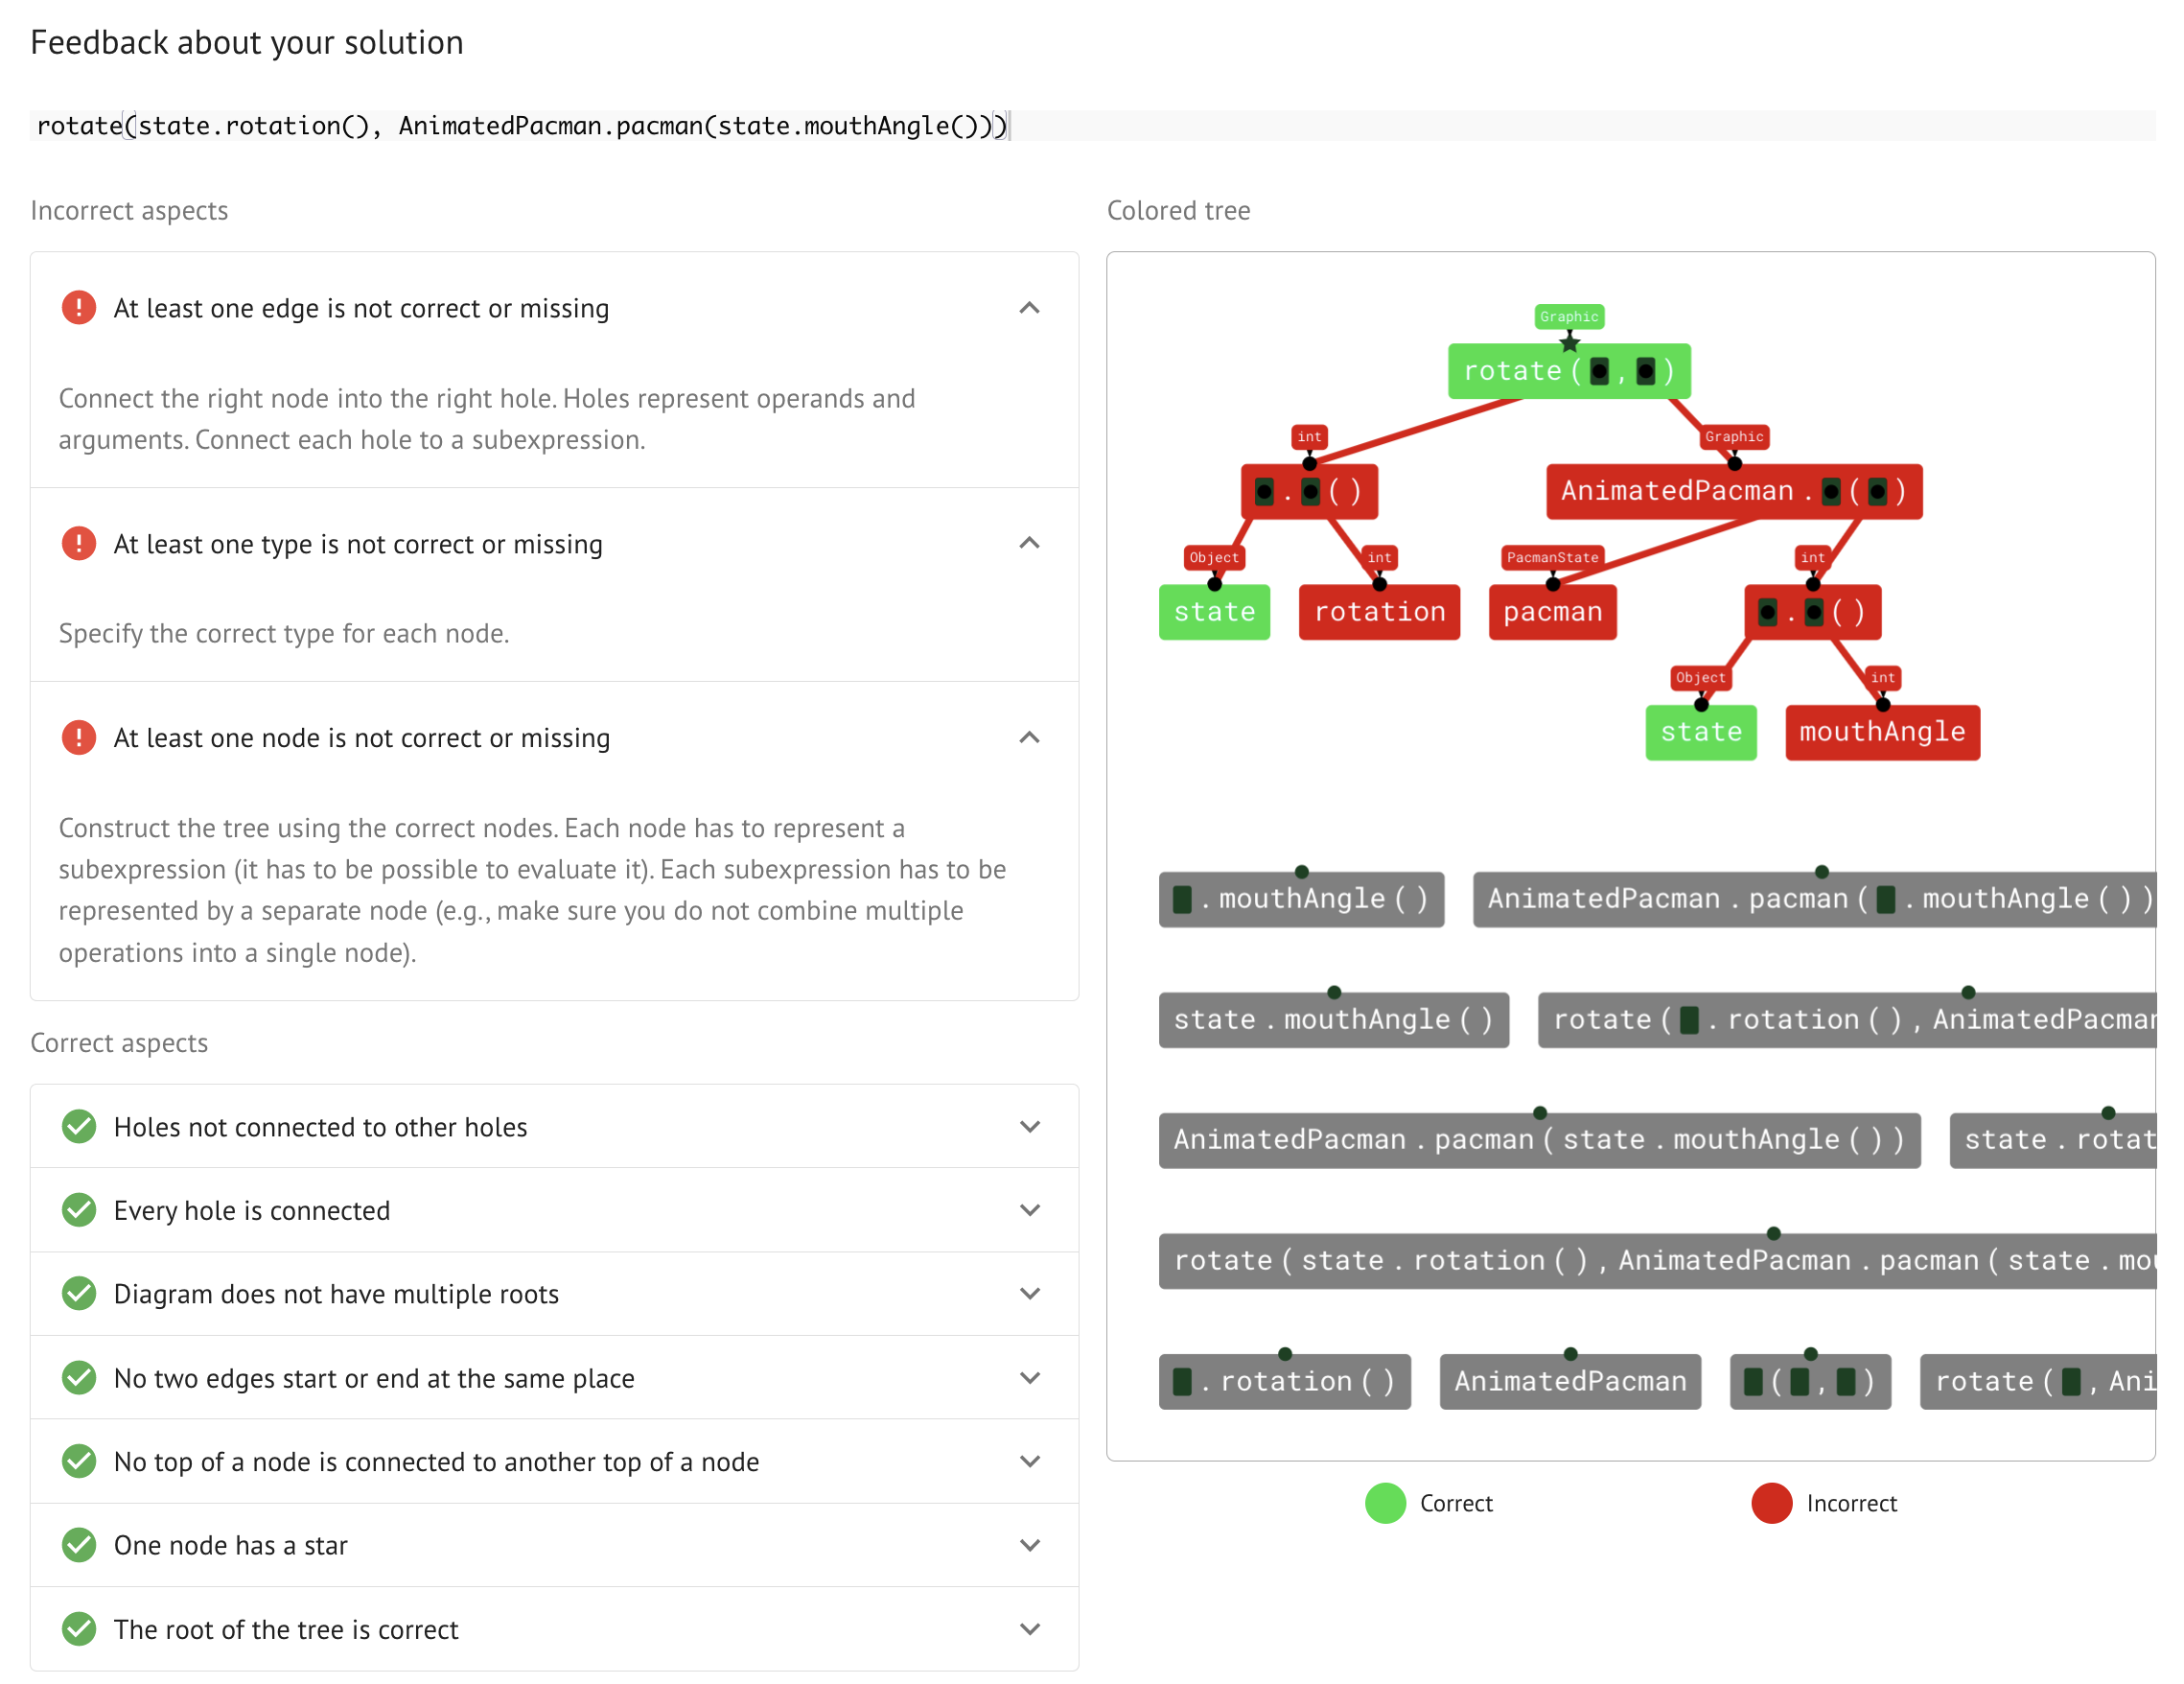
\includegraphics[width=\textwidth]{res/7/ff_example.png}
    \caption{Example of formative feedback provided to students upon
submission of an Expression Tutor activity.}
    \label{fig:fb-ff-dialog}
\end{figure}

\subsection{Implementation}

The generation of the formative feedback is based upon the Assessment
capabilities of the platform. The coloring of the student's submission
leverages the diagram–coloring algorithm described previously in
\textbf{Section~\ref{sec:fb-assess-color}}.

Both components of the formative feedback are generated by leveraging
the assessment report produced by the assessment system
(Section~\ref{sec:fb-assess}). The \textit{coloring} information is
used to color the submission to allow the student to quickly visualize
the structural incorrectness. The properties also provide feedback that is
relevant for structural correctness. By expanding the description of a
property, the student can read a description that explains why violating
such property is wrong and is given a hint towards a correct solution.
Some of the properties are directly taken from the tree–well–formedness
properties described in Section~\ref{sec:fb-assess-tree}, although they
are presented with different terminologies to hide the implementation
details students should not be concerned with so that the descriptions
and hints can focus more on the concepts that are relevant to the
learning goal of understanding expressions through the use of the
Expression as Trees notional machine.

Students may only receive feedback after saving their submission, even
though the system would have worked just as well with a non–saved
submission. Moreover the submission may still be changed after being
saved, so students can make use of the information gained from the feedback
to improve it.
The design choice of allowing students to receive feedback only after
saving was made so that they would not abuse the feature to \textit{game}
the system and turn the Expression Tutor activity into an exercise of
mindlessly \textit{turning all the lights green}. Adding additional
artificial friction to obtain the feedback by having to \textit{save}
the submission, makes the student less likely to abuse this function and
spend more time reasoning about their submission without being too reliant
on the automated feedback. The downside of this decision is that feature
discoverability is decreased. If the feedback was always available during
the completion of the Expression Tutor activity, it would be more frequently
utilized, and could help more students catch and correct certain mistakes
and misconceptions earlier. Moreover, it is possible for people who are
less invested in the learning experience to never engage with the
feedback functionality once they have saved their submission because for
them it may not be worth the \textit{effort} to go back and correct a
mistake, unless there is some additional external incentive or
reward for doing so.

\subsection{Evaluation}

To evaluate the quality and efficacy of the formative feedback feature
implemented in Expression Tutor activities, we asked a number of
students who were given as additional non–graded homework exercises
Expression Tutor activities automatically generated starting from
code from their own assignment submissions.
The evaluation consisted of the following questions:

\begin{enumerate}
    \item Did you complete any of the Expression Tutor activities that
were posted in your lab repositories on GitHub?
    \begin{itemize}
        \item Yes, the most recent one during the last week
        \item Yes, the most recent one before the last week
        \item No, never
    \end{itemize}
    \item Were you aware of the automatic feedback feature? If so,
did you use it?
    \begin{itemize}
        \item I was aware of it and I did use it
        \item I was aware of it but I did not use it
        \item I was not aware of it and I did not use it
    \end{itemize}
    \item If you used it, did you find it useful? Why? Which
particular aspect of it was most helpful to you?
    \item If you used it, which particular aspect of it was not
very helpful to you?
    \item Do you have any suggestion regarding the automatic feedback
feature?
\end{enumerate}

94\% of the respondents had completed at least one of the automatically
generated Expression Tutor activities. Among those, the 62\% of them
was aware of the possibility of receiving automatic feedback for their
submission. Of them, only the 55\% actively made use of the feedback
functionality.

Students appreciated being able to access visual feedback that displays the
wrong or incomplete parts of their tree. In particular, multiple students
reported the feedback helped them remind of labeling the expression tree with
the types of each node.
As downsides to the implementation of the formative feedback on the Expression
Tutor website, the main issue that was raised was the fact that the feature is
easy to miss or forget about when saving a submission. This is reflected in the
significant percentage of people who stated that they were not aware of the 
existence of such functionality (44\% among those that had completed at least one
Expression Tutor activity).

This evaluation tells us that the feedback feature needs to be made more easily
discover–able on the platform so that more students can benefit from it.
Instructors can also help by pointing out to students that the Expression Tutor
platform allows them to obtain feedback.
Moreover, a more detailed experiment is need to evaluate the specific aspects
of the feedback provided to students.

\section{Feedback for Instructors}\label{sec:fb-sf}

While students are concerned with understanding whether their individual
submission was correct (and in case it was not, what was wrong about it), 
instructors may find it more insightful to understand the performance of the
overall group of students.
By accessing the \textit{Report} section of activity groups
(Section~\ref{sec:impl-agi}), instructors can obtain summarized information
about all the different submissions of students.

The activity group report user interface is divided into three different
main sections. The first section, labeled \textit{Overview} (as seen in
\textbf{Figure~\ref{fig:fb-sf-overview}}), displays key information about the
activity group. Depending on the configuration of the activity group, the
contents of this section may vary. For activities which have one shared
reference solution, the expression tree of said reference solution is visualized
at the top (as seen in Figure~\ref{fig:fb-sf-overview}).

In case the activity group contains activities with multiple different
reference solutions, instead less accurate information about the submissions
status is displayed.
As argued in Section~\ref{sec:impl-agi-ag}, if each student has its own unique
reference solution, then it becomes possible to reliably know how many different
activities were generated and how many had at least one submission. If all
submissions stemmed from the same original base activity and thus share the same
reference solution, then it is not possible to obtain such information due to the
lack of any form of \textit{student identification} by design on the Expression
Tutor platform. 
At the top of this page, the query associated to the activity group is also
shown to provide additional context as to how the activities were generated.

Below that, the page presents up to four different submissions as highlights
among all of the submissions that belong to the activity group. These
highlighted submissions serve to bring to the instructor's attention diverse
submissions with different \textit{grade of correctness}. The selection of
these submissions that are showcased is performed by making use of a technique
called stratified sampling~\cite{parsons_stratified_2017}.
Stratified sampling allows to sample a diverse population by sampling
each sub–population (stratum) independently. The stratification process
consists of dividing the members of the population into multiple homogeneous
subgroups before sampling them.
We begin selecting all the submissions with unique contents (uniqueness
determined by computing an hash value of the entire ExpressionTreeDiagram
instance) to constitute the population to be sampled. The different diagrams
are then divided into different strata. 
In this particular instance, the population made of different submissions
(uniqueness determined by an hash value computed on the expression tree diagram)
is divided into strata depending on the respective \textit{grade} value
(Section~\ref{sec:fb-assess-grade}). From each stratum we sample a number of
submissions randomly. The number of the selected entries depends on how many
submissions we want to showcase and how in how many strata were used.
This number is not selected proportionally to the size of each strata
because we want the sampled activities to not be very similar to cover more
different scenarios with the least number of submissions.

The second section, labeled \textit{Incorrect nodes} provides a summary of all
of the incorrect nodes that were found in during the assessment process, as
illustrated in \textbf{Figure~\ref{fig:fb-sf-incorrect-nodes}}. This information
is particularly useful, even when submissions have different reference 
solutions.
By looking not only at which, but also how many times the incorrect distractor
nodes were included in the submissions of students provides the instructor with
information about concepts that were not understood. If, for instance, in an
Expression Tutor activity based on expressions written in the Java programming
language, the incorrect node \lstinline[language=etl]{(() "." () "(" () ")")}
appears many times even though the students were supposed to compose trees for
expressions involving only static method invocations, it means that there is 
some misconception about how static method invocation works. This list includes
both nodes that were classified in the $ S $ and $ R $ sets described in
Section~\ref{sec:fb-assess-nodes} and not only those incorrect nodes found in 
the submissions of the students (set $ S $). Highlighting the incorrect nodes 
in the $ R $ set can also help instructor understand the misunderstanding and
misconceptions that students have. The information provided in this section is
also made available for download as a CSV (Comma–Separated–Values) file,
offering a convenient way to plug this data in other external systems.

The third section, labeled \textit{Assessment}, offers a more comprehensive
view of all the information generated by the assessment system organized in
a table, as seen in \textbf{Figure~\ref{fig:fb-sf-assessment-table}}. Each
row of table represents one different submission and can be expanded.
Upon expansion, more details about the submission are revealed, as
illustrated by \textbf{Figure~\ref{fig:fb-sf-assessment-details}}. The
details offer the instructor the possibility of visualizing the student's
submission and its respective reference solution colored (according to
Section~\ref{sec:fb-assess-color}) and the linearization 
(Section~\ref{sec:fb-assess-linearization}) of the two. The table entries
may be sorted for any of the columns for convenience. The data presented
in this table is also made available for download in both CSV and JSON format,
offering a convenient way to make use of the data produced by the assessment
report in other external systems with ease.

The submissions of the students, unlike the reference solutions, are
visualized with the exact same layout as the student saved them. While this
seems like a minor relatively–important thing, it is instead worth pointing
out how, the positioning of various nodes captures additional information
about how the student perceived the tree, allowing to communicate to the
instructor more information than just that provided by looking at the raw
diagram data  structure. One such example would be when there are diagrams
that are not well–formed trees. Just looking at the layout of nodes in the
student's submission can help shed some light on the reason why the diagram
has the \textit{shape} it has, and can help identify more mistakes and
misconceptions that particular student might have.

\begin{figure}[ht]
    \centering
    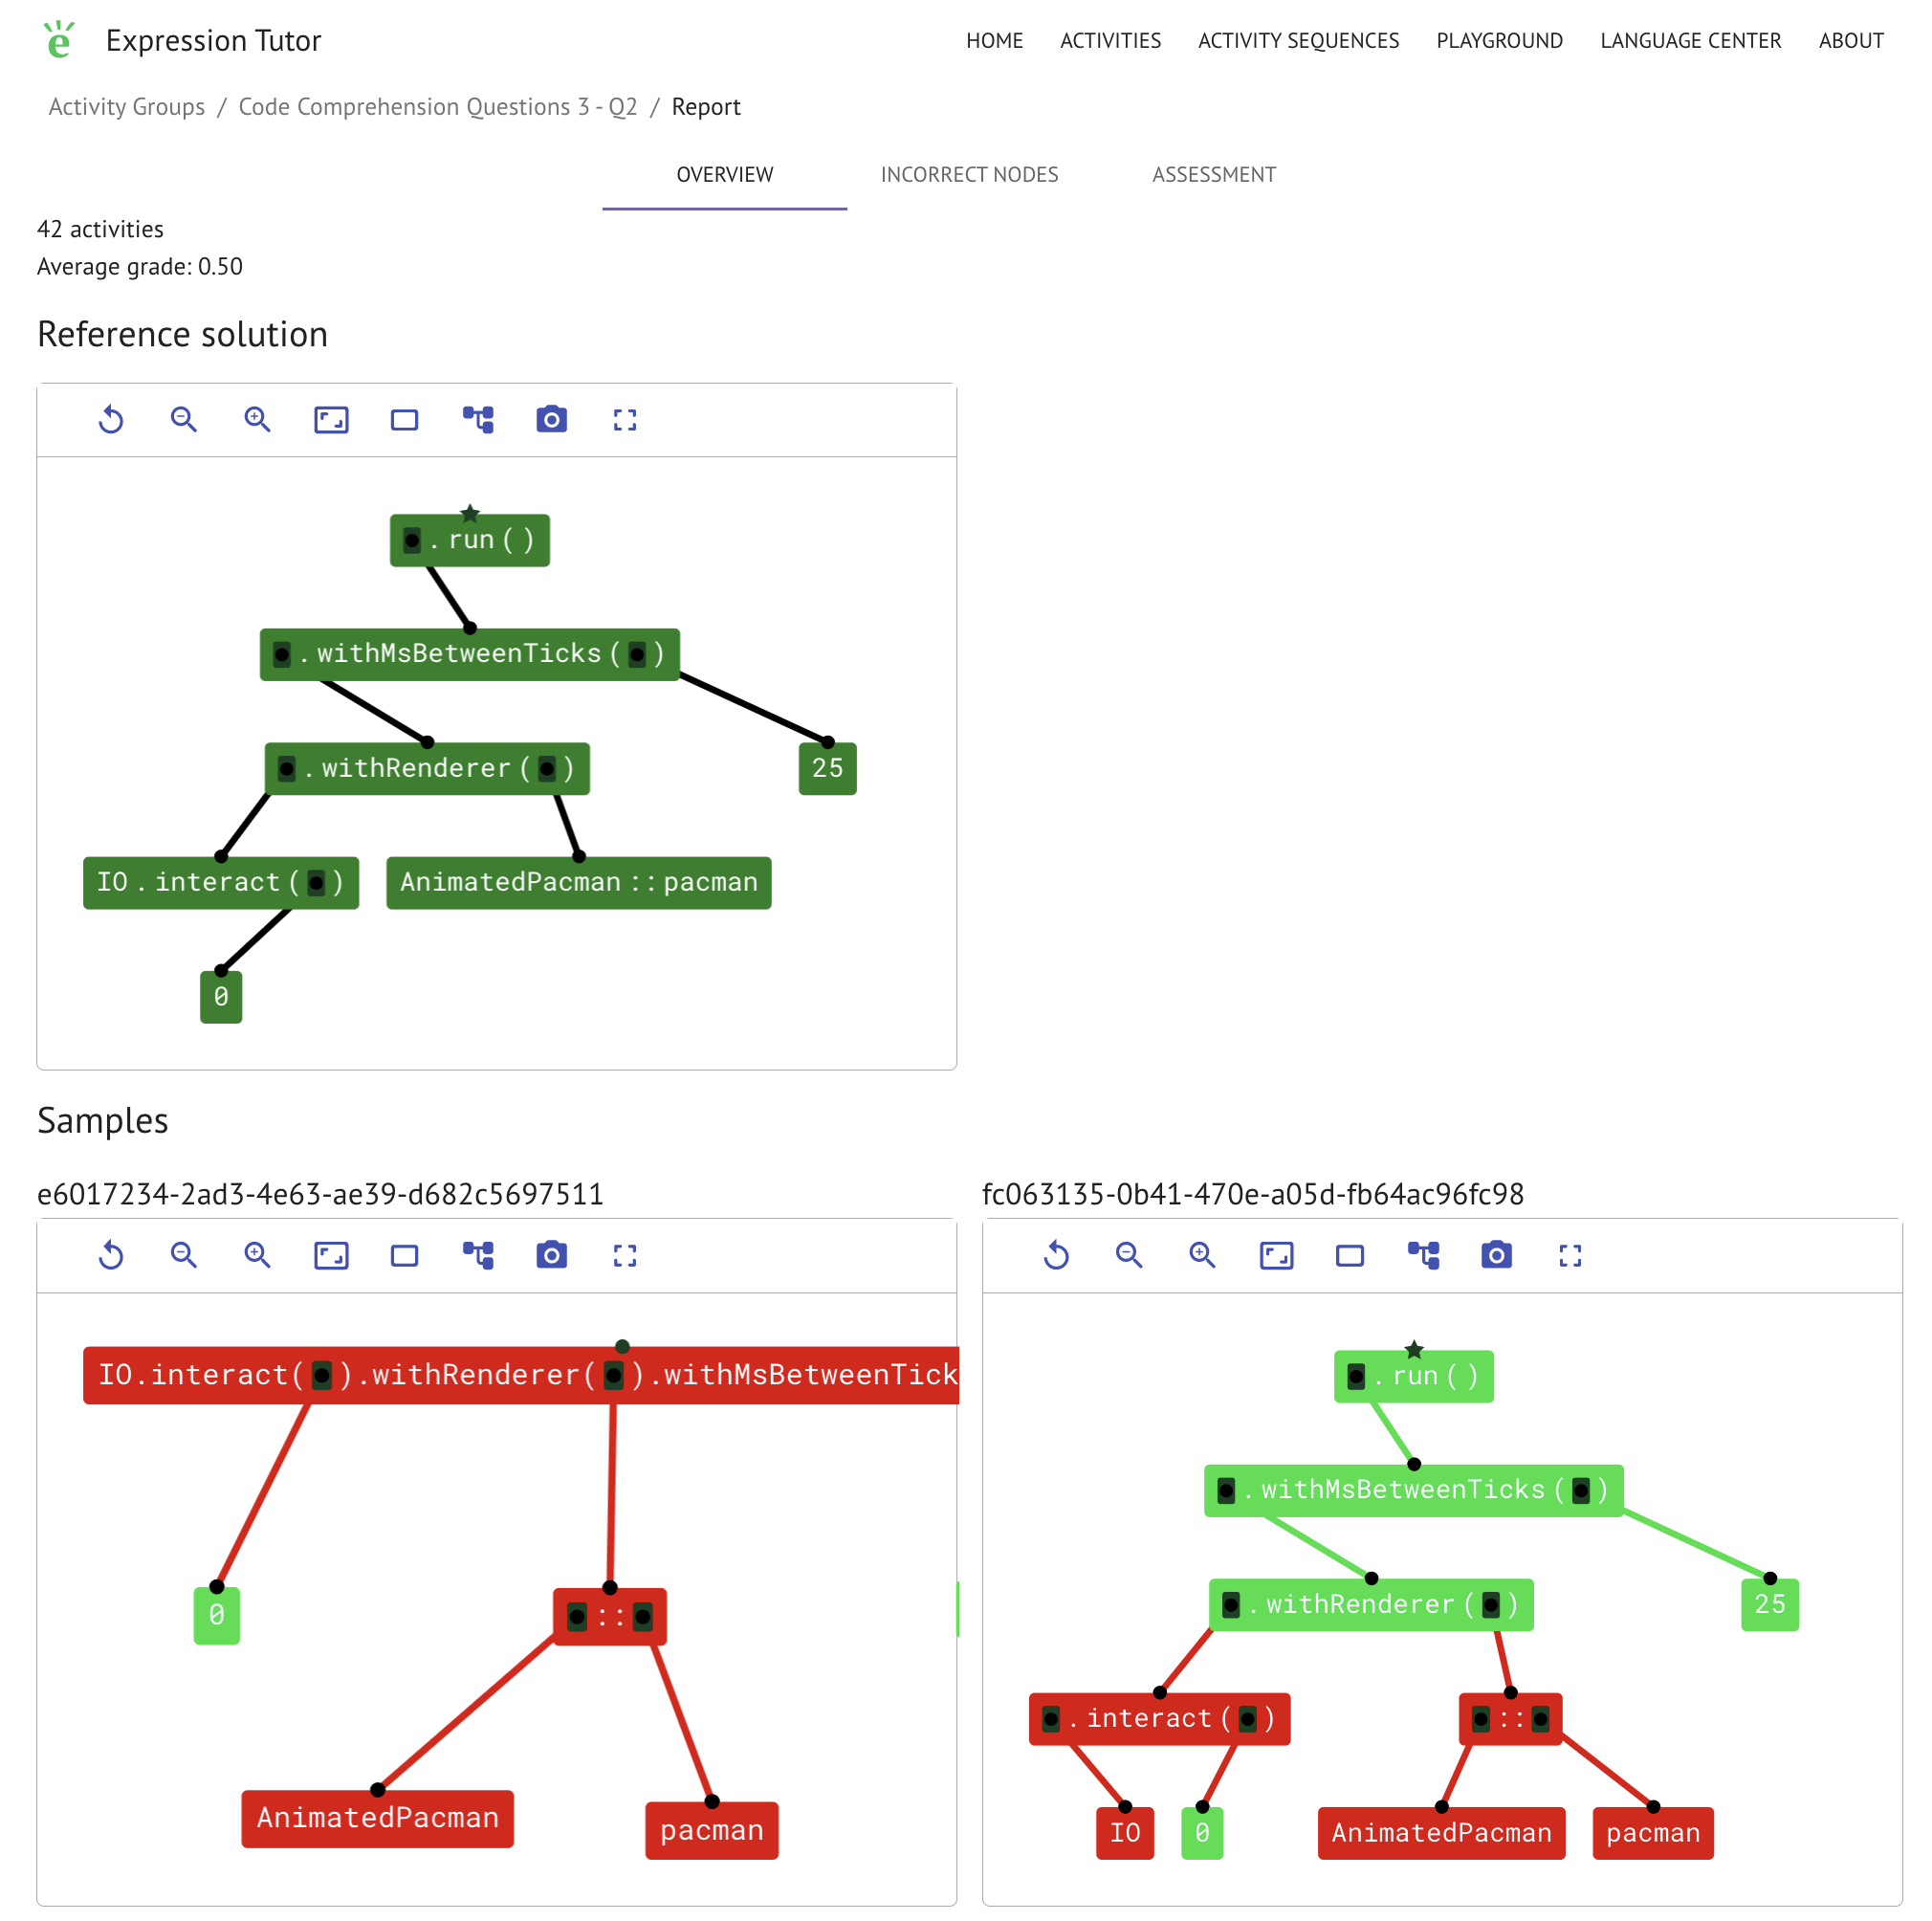
\includegraphics[width=\textwidth]{res/7/sf_overview_same_refsol.png}
    \caption{Overview of the feedback for an activity group.}
    \label{fig:fb-sf-overview}
\end{figure}

\begin{figure}[ht]
    \centering
    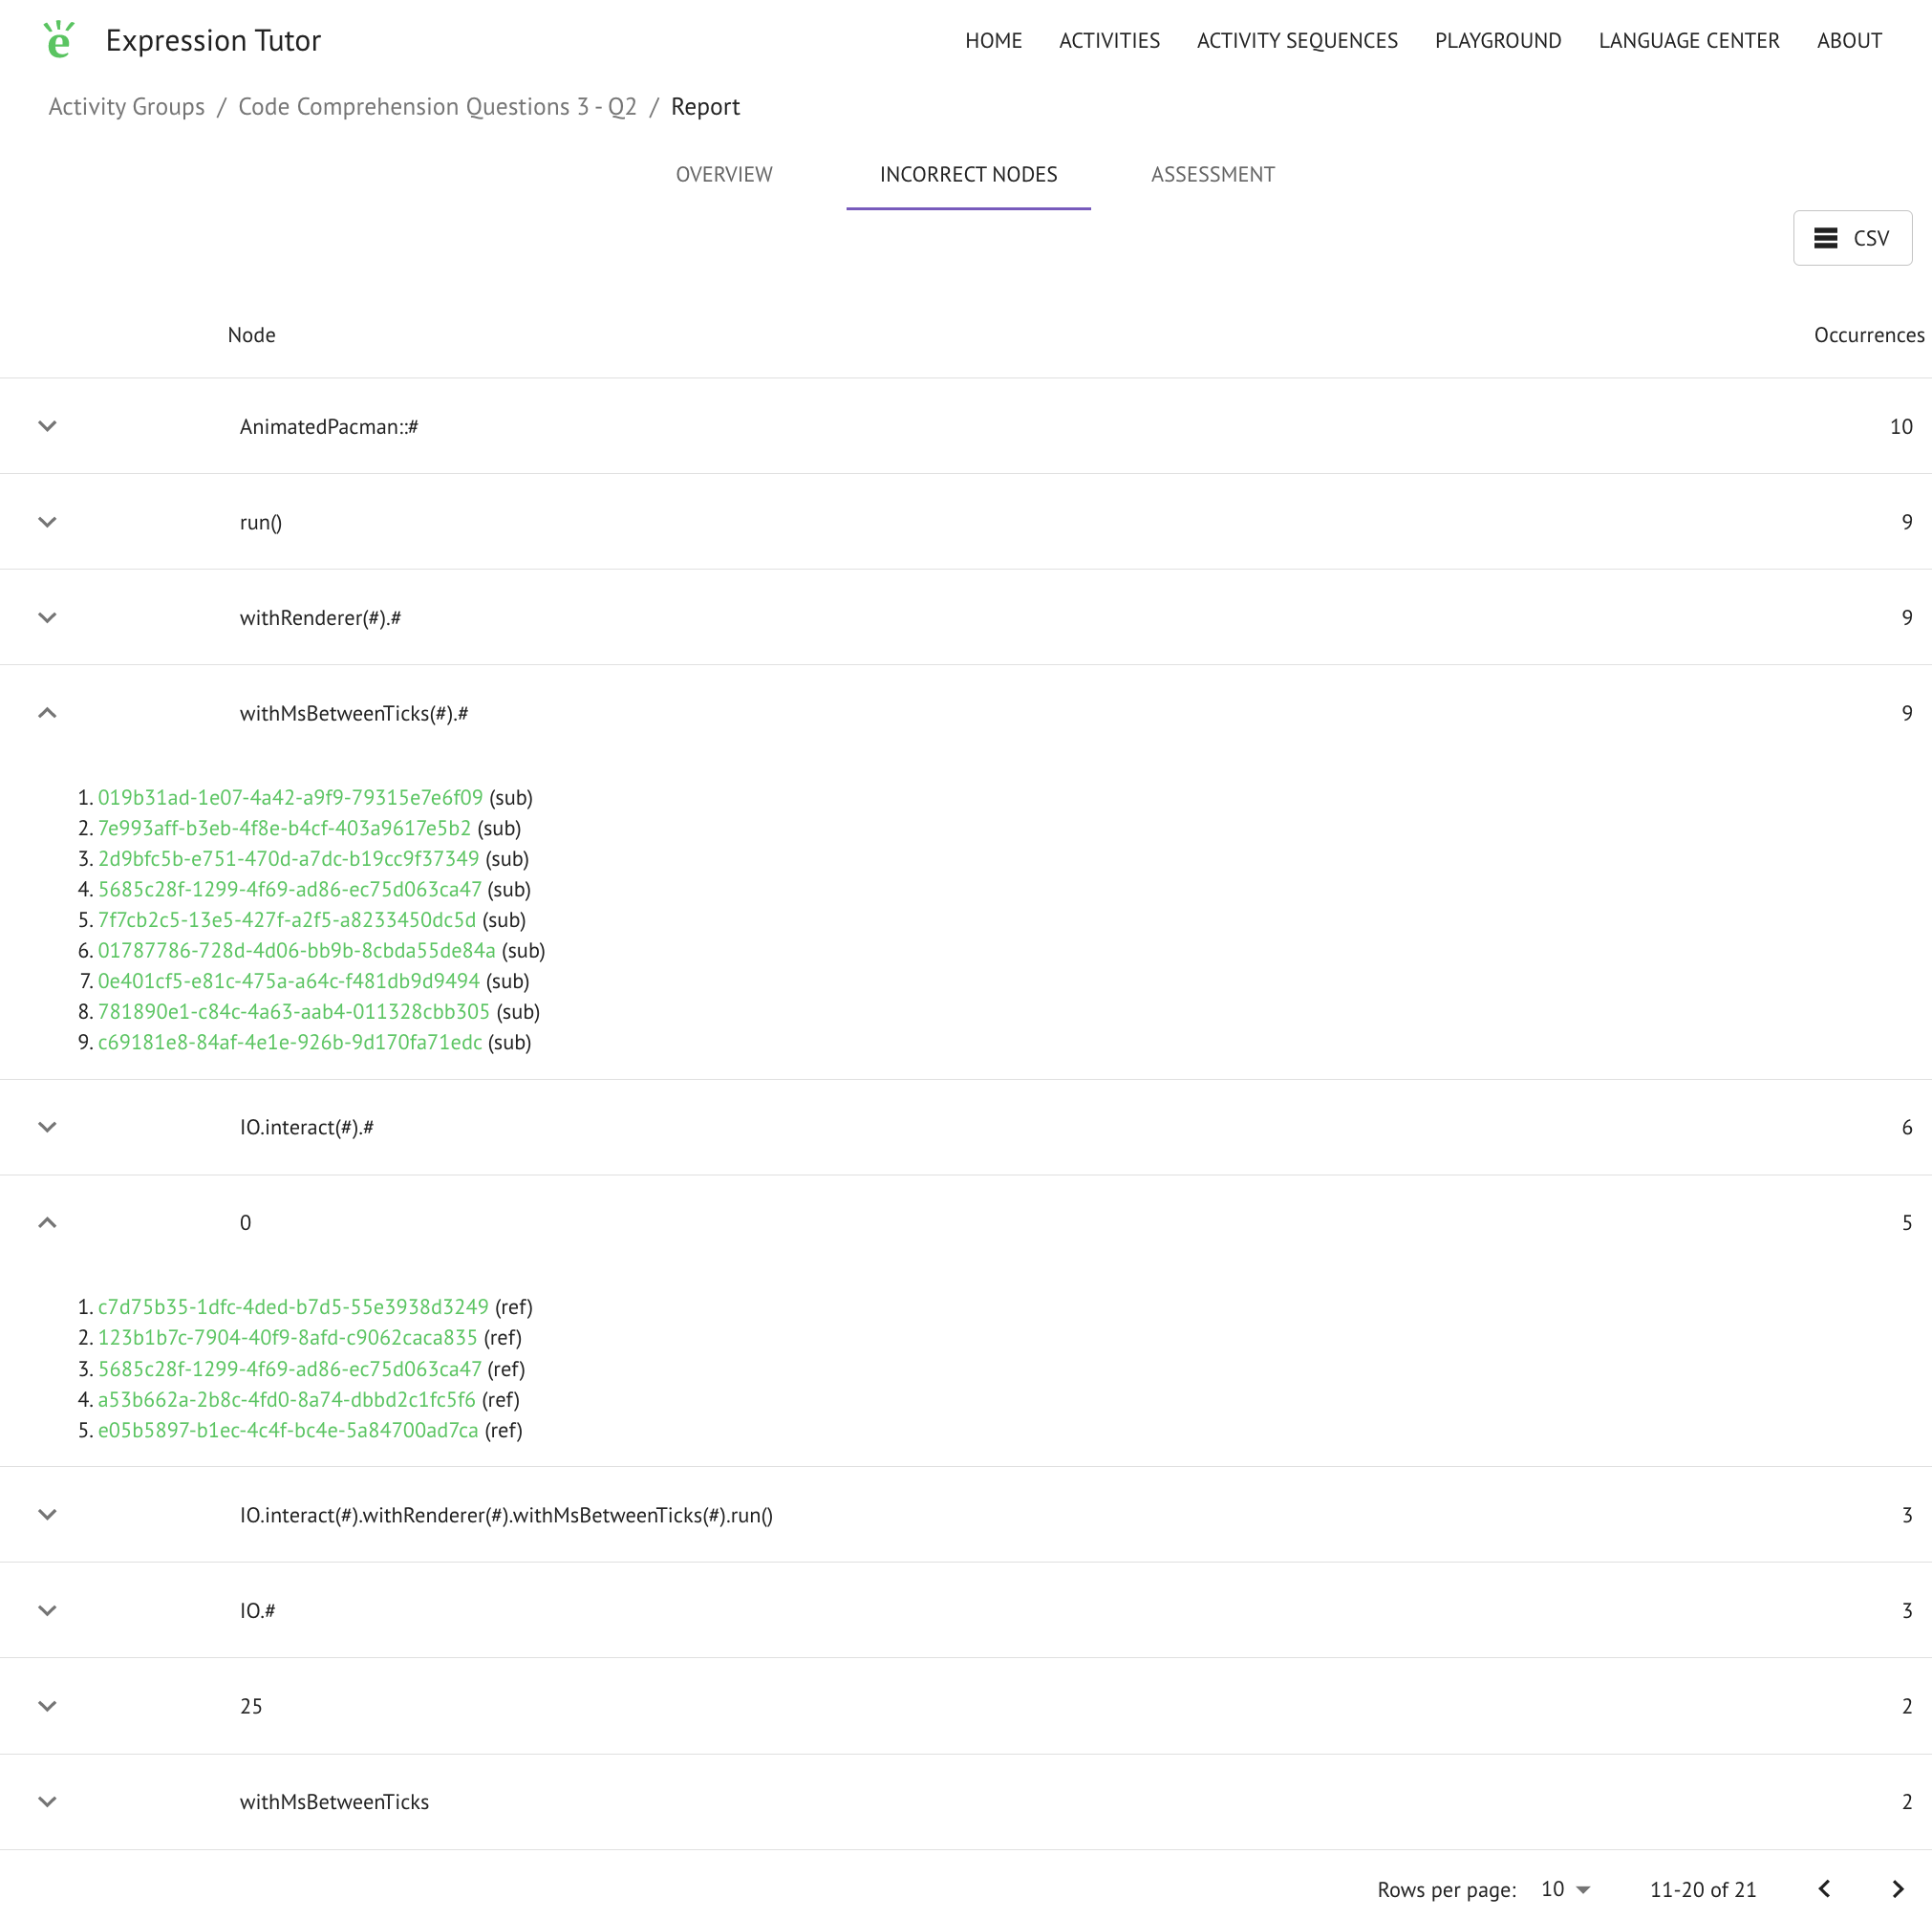
\includegraphics[width=\textwidth]{res/7/sf_incorrect_nodes_table.png}
    \caption{Incorrect nodes that appeared in all the activities of an activity
group.}
    \label{fig:fb-sf-incorrect-nodes}
\end{figure}

\begin{figure}[ht]
    \centering
    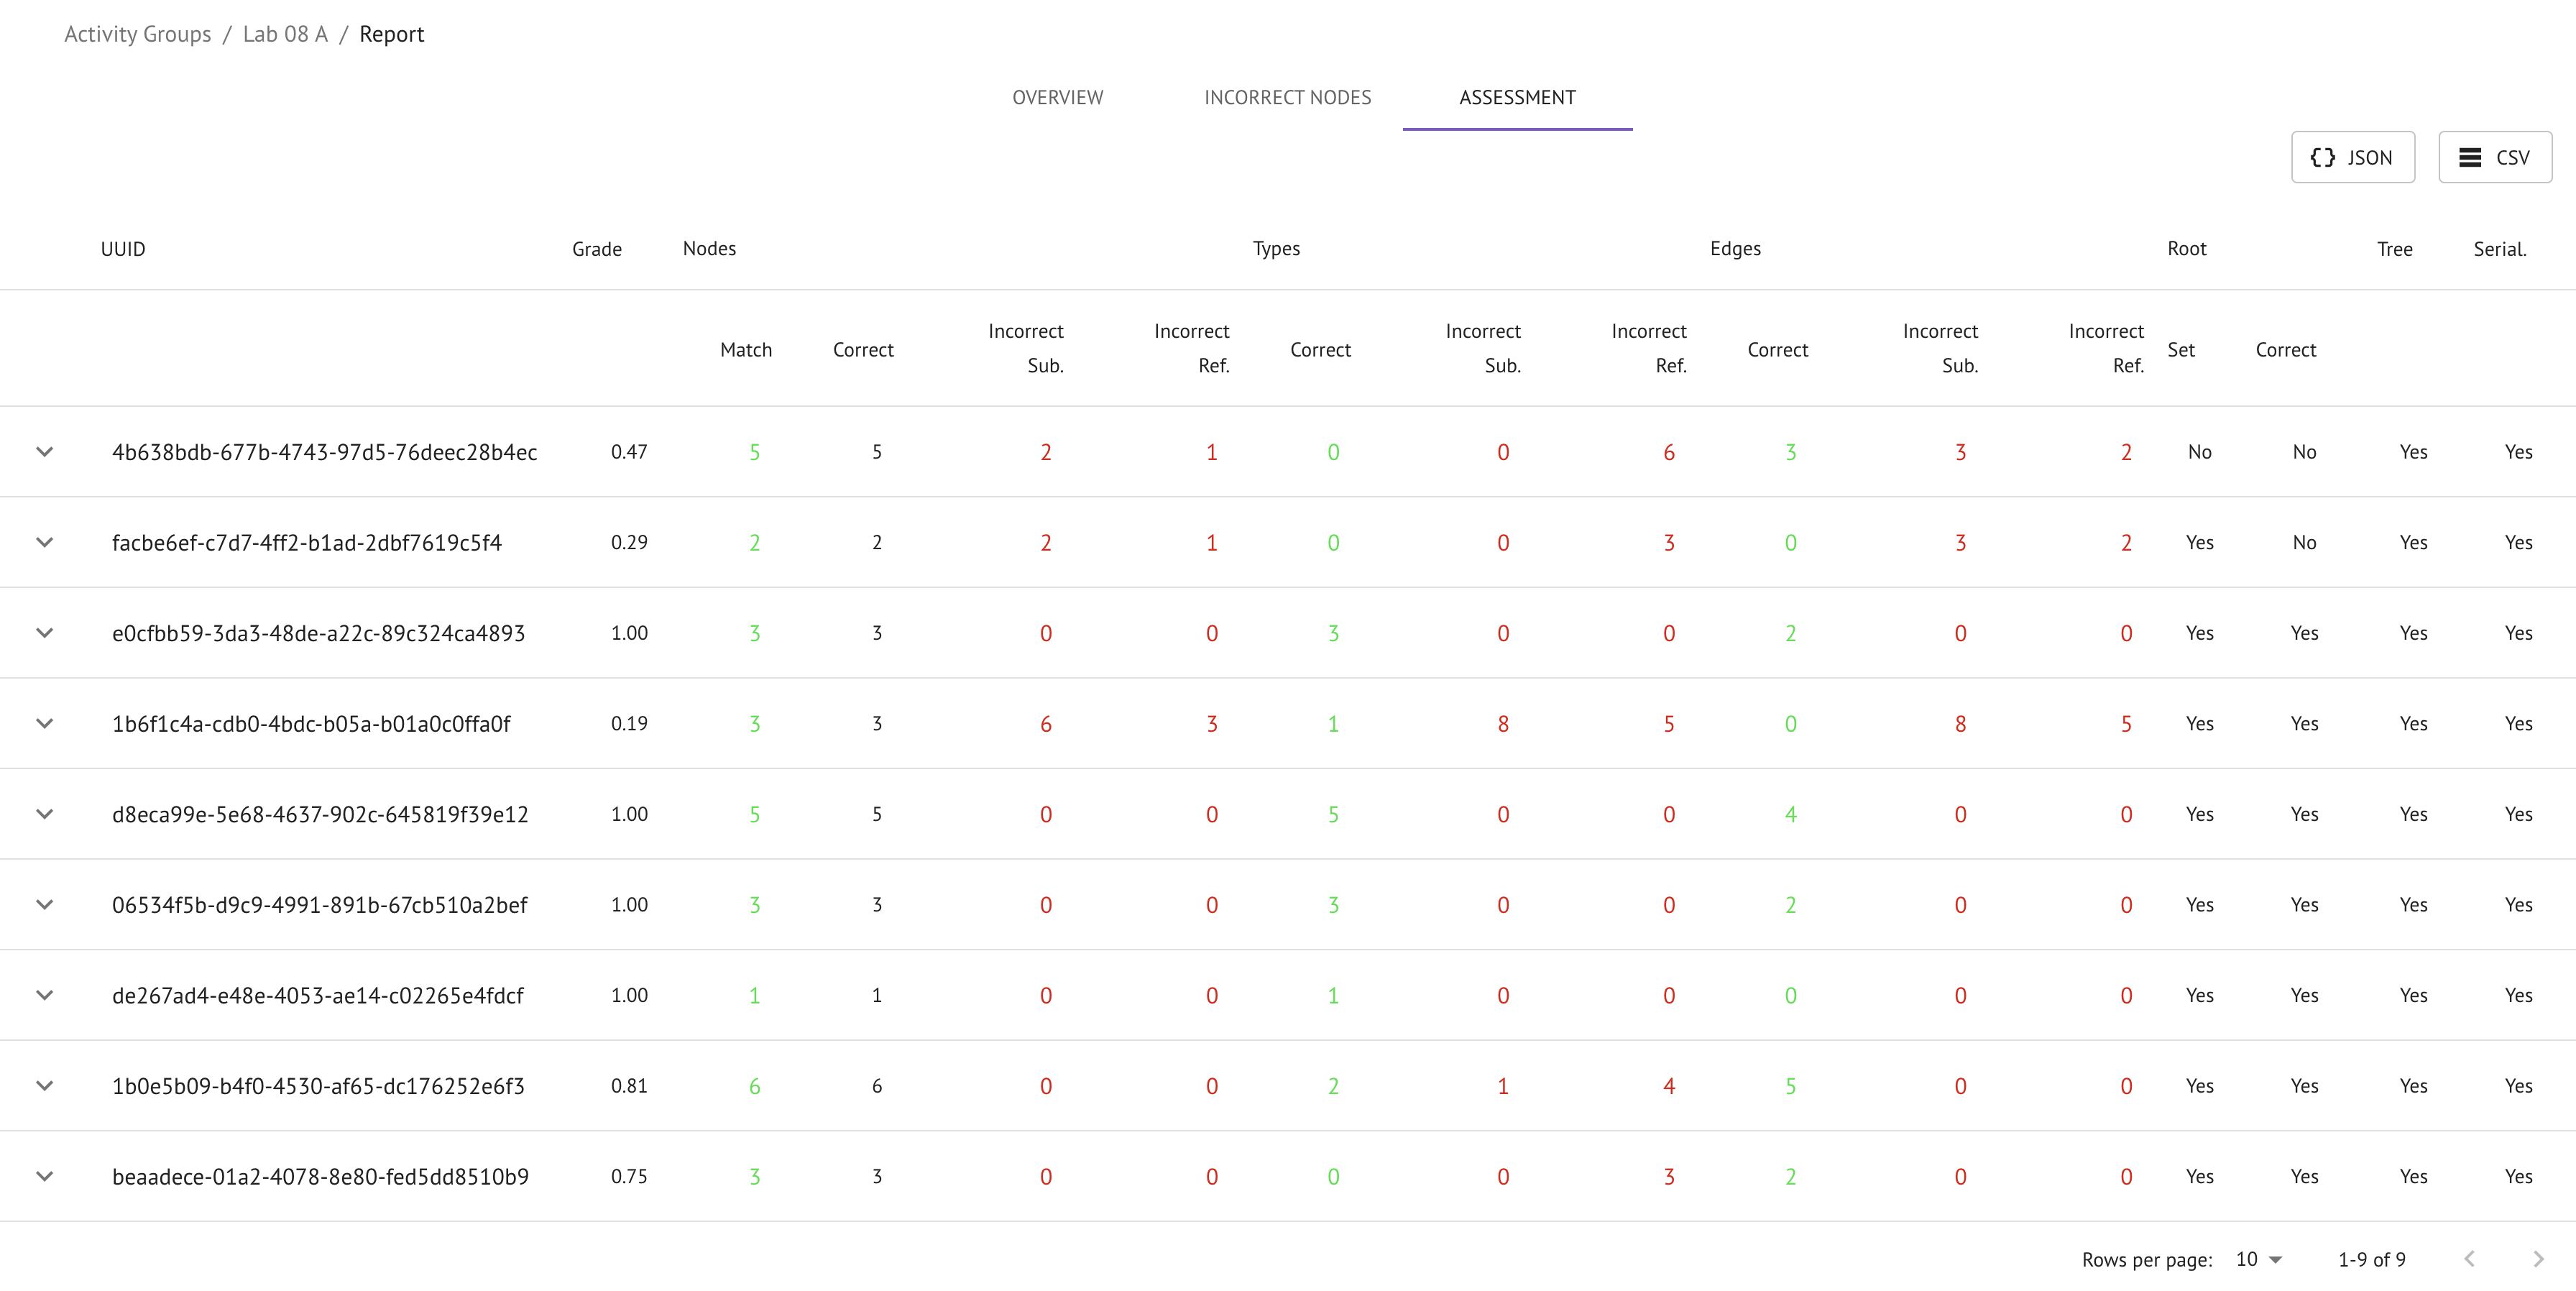
\includegraphics[width=\textwidth]{res/7/sf_assessment_table.png}
    \caption{Assessment table of an activity group.}
    \label{fig:fb-sf-assessment-table}
\end{figure}

\begin{figure}[ht]
    \centering
    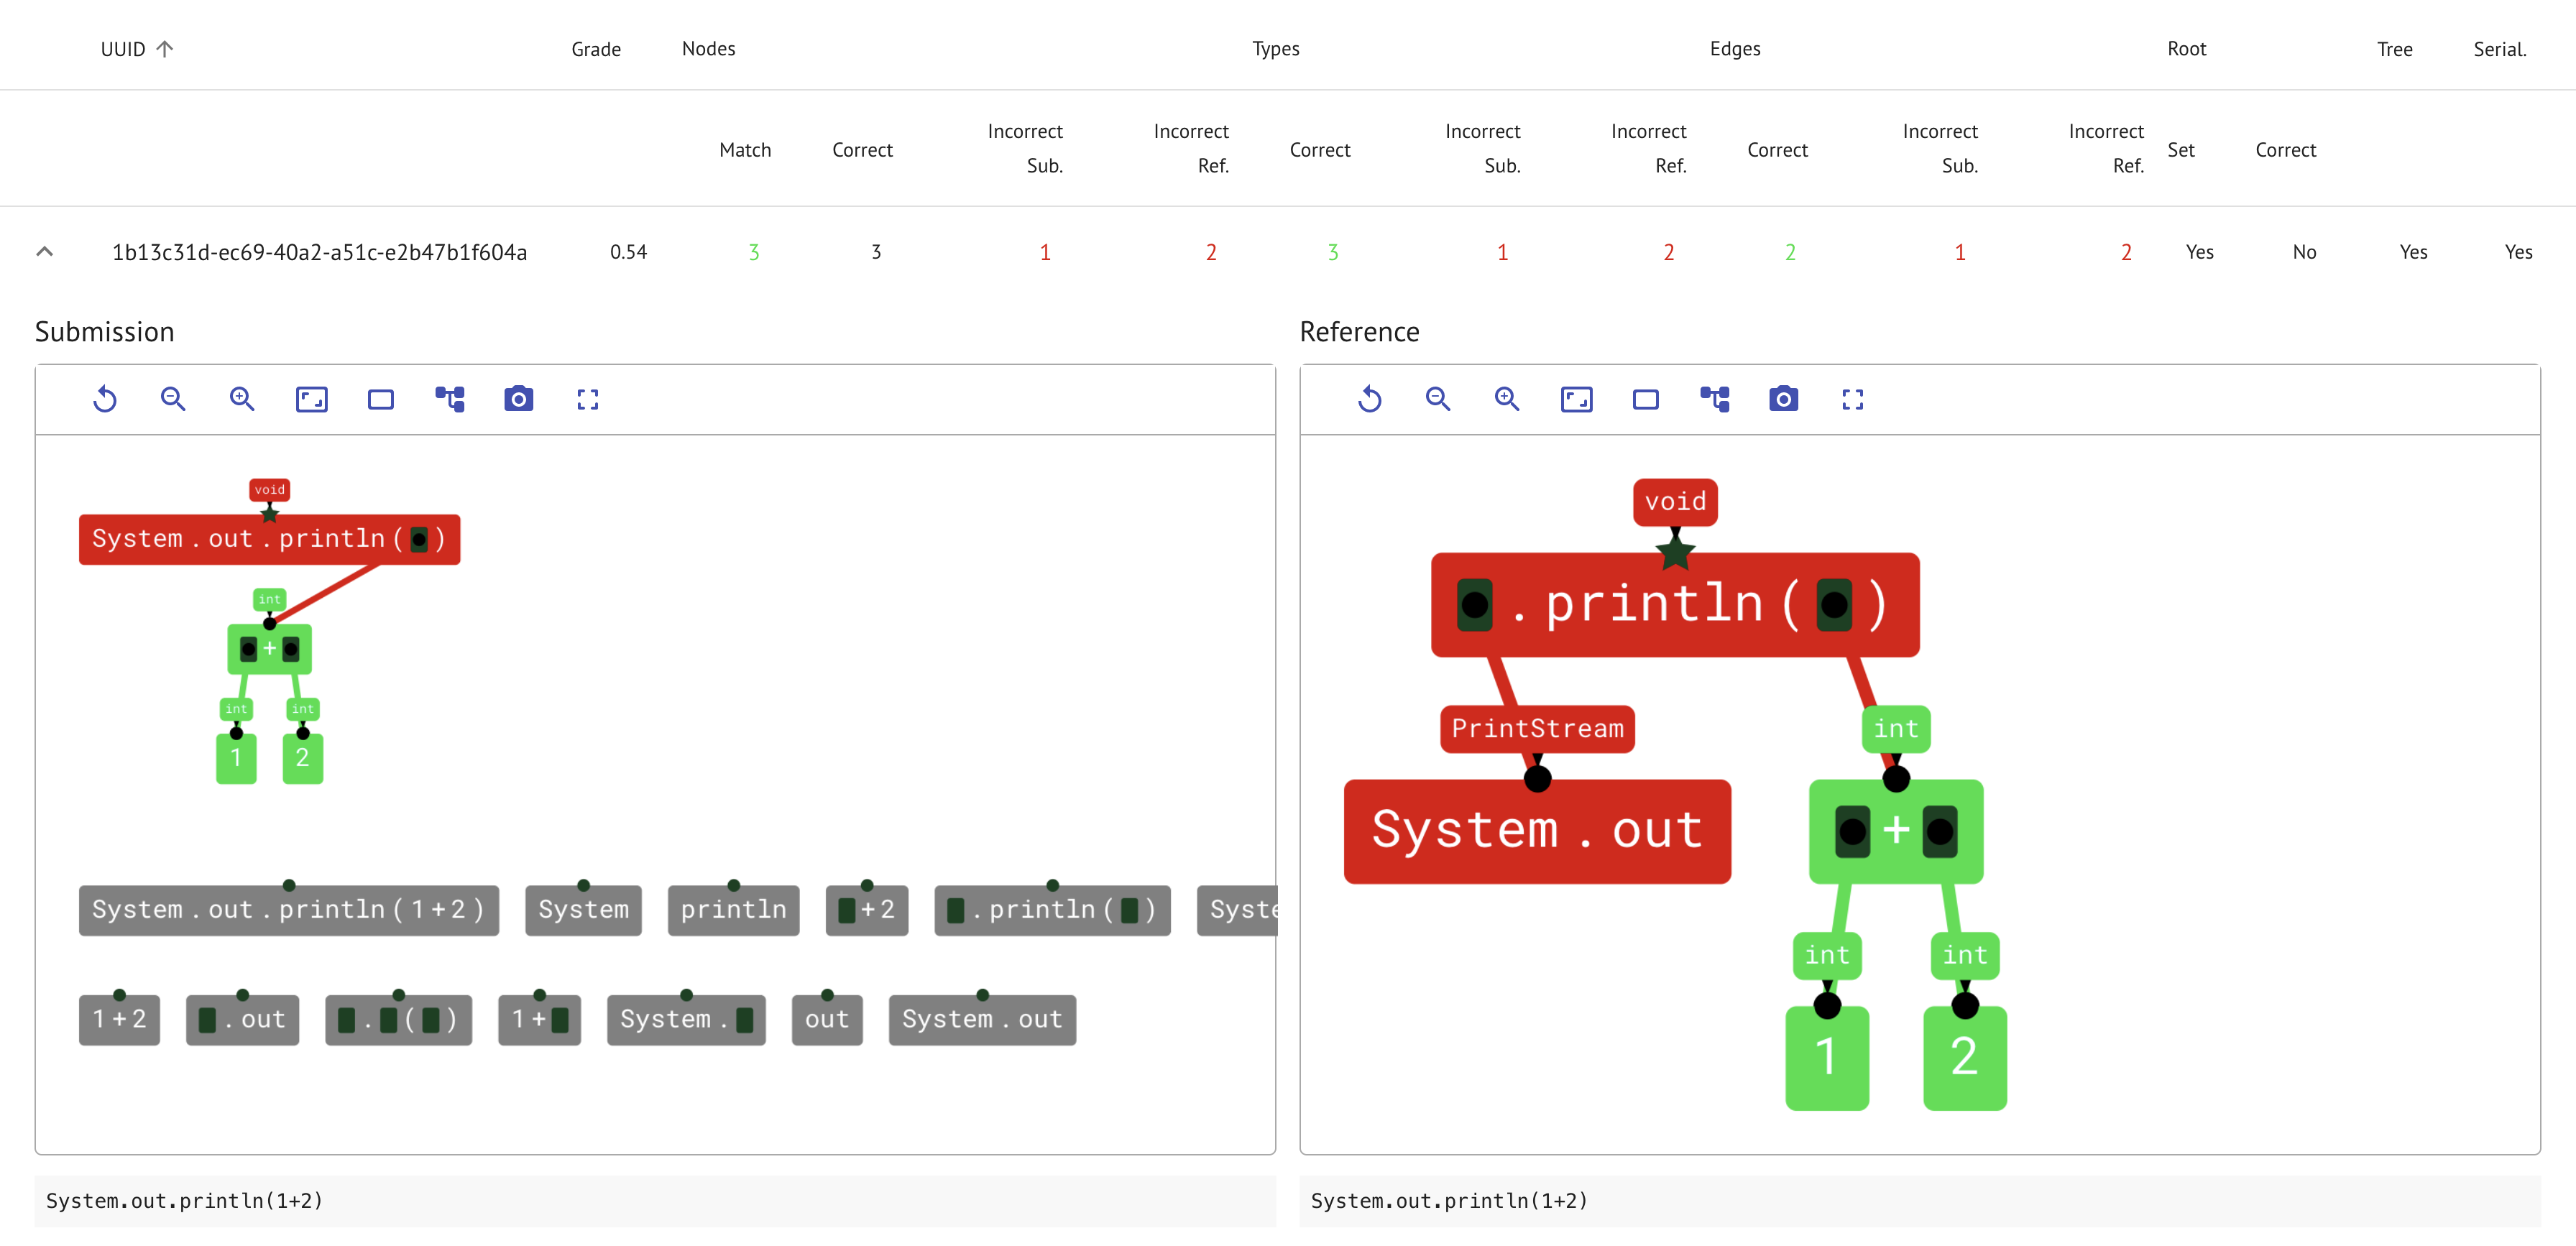
\includegraphics[width=\textwidth]{res/7/sf_assessment_individual.png}
    \caption{Details of an activity submission in the assessment table.}
    \label{fig:fb-sf-assessment-details}
\end{figure}

\end{chapterBody}
